\section{State of the Art}

This section presents an overview of the state-of-the-art in the realm of single-trial functional connectivity within EEG-based motor imagery brain-computer interface systems. Our focus is on the cutting-edge approaches designed to tackle the problems described in \cref{sec:problem_statement}, with a subsequent discussion addressing their respective strengths and drawbacks. Initially, we explore single-trial FC feature extraction and estimation. Following this, we discuss end-to-end models that merely depend on the raw EEG data. Lastly, we provide a comprehensive outline of the different interpretability strategies, focusing on deep learning. This overview will allow the reader to comprehend new strategies to clarify the underlying complexities of single-trial FC and its critical role in EEG-based MI-BCI systems.


\subsection{Single-Trial FC in MI-BCI \label{sec:sota1}}

In the context of MI-BCI systems, using FC estimators becomes crucial in decoding the intricate links between different brain parts during MI tasks. These linear and non-linear estimators attempt to measure the statistical dependencies between neurophysiological recordings from different regions, providing crucial insights into brain mechanisms. In addition, FC-based feature extraction techniques play a significant role in effectively translating the nuanced connectivity information into distinguishable patterns related to different MI tasks. When properly extracted and processed, these features enable improved classification and prediction in MI-BCI systems. Over the years, numerous studies have delved into the exploration and enhancement of FC in MI-BCI, leading to significant advancements and understanding. Yet, the field presents challenges and opportunities, particularly considering the complexities and variabilities inherent to brain function and MI processes.


\subsubsection{Functional Connectivity Estimators}

This section offers a review of the most commonly used functional connectivity estimators in the field of EEG-based BCI systems, highlighting their utility and relevance. Given the range of available brain connectivity estimators, selecting an appropriate one is a critical initial step when working with single-trial FC in EEG-based MI-BCI systems. These estimators can generally be broadly categorized based on several factors. First, the domain of interest can be either time or frequency. Second, whether the connectivity is direct or indirect, the former referring to simple zero lag correlation and the latter about the k-lag or cross-correlation. Third, whether the interactions are grounded in a linear or nonlinear formulation. A detailed representation of these categorizations can be found in \cref{fig:sota1_FC}.

\begin{figure}[h]
    \centering
    \resizebox{\linewidth}{!}{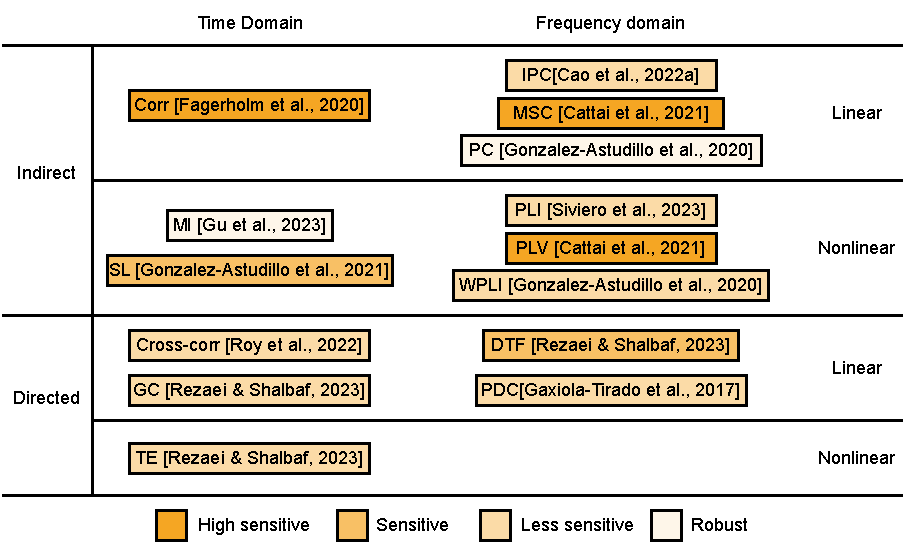
\includegraphics{Figures/state_of_art/sota1_EFC.pdf}}
    \caption{Functional connectivity estimators classified based on direct or indirect, time or frequency domain and linear or nonlinear. The varying shades of orange represent different sensitivities to volume conduction, with lighter shades indicating a higher degree of robustness and solid ones indicating a high level of sensitivity. Abbreviations: Corr, correlation \cite{fagerholm2020dynamic}; MSC, magnitude square coherence \cite{cattai2021phase}; IPC, imaginary part of the coherence  \cite{cao2022brain}; PC, partial coherence \cite{gonzalez2020network}; PLI, phase lag index  \cite{siviero2023functional}; WPLI, weighted phase lag index \cite{gonzalez2020network}; PLV, phase locking value \cite{cattai2021phase}; MI, mutual information \cite{gu2023decoding}; SL, synchronization likelihood \cite{gonzalez2021network}; Cross-corr, cross-correlation \cite{roy2022comparative}; GC, Granger causality \cite{rezaei2023classification}; TE, transfer entropy \cite{rezaei2023classification}; DTF, directed transfer function \cite{rezaei2023classification}; PDC, partial directed coherence\cite{gaxiola2017using} \label{fig:sota1_FC}}
\end{figure}


Linear estimators, due to their straightforward computation and interpretability, have been widely investigated for predicting brain connectivity in MI-BCI systems \cite{gonzalez2020network, van2015opportunities}. The simplest method of estimating linear intercommunication between EEG signals is based on the widely recognized Pearson correlation (Corr) for indirect connectivity and cross-correlation (Cross-corr) for direct connectivity \cite{fagerholm2020dynamic}. It's important to note that Cross-corr is essentially an expanded version of correlation (zero time lag) that considers a k-time lag. As a result, the correlation may not accurately represent linear relationships if there is a delay between specific patterns from two EEG channels \cite{roy2022comparative}. A frequency domain counterpart of correlation is coherence, which is based on the amplitude synchrony of the Power Spectrum Density (PSD) between two EEG signals \cite{cattai2021phase}. Specifically, Magnitude Squared Coherence (MSC), and the Imaginary Part of Coherency (IPC) are two coherence-based FC estimators that are widely used, with the latter being less sensitive to the volume conduction problem \cite{cao2022brain}. While most of the FC estimators rely on the interactions between two signals without removing the influence of other signals, Partial Coherence (PC) and Partial Directed Coherence (PDC) are designed to alleviate spurious connectivities due to common influence from other signals \cite{gonzalez2020network}. Additionally, Directed Transfer Function (DTF) in the frequency domain and Granger Causality (GC) in the time domain employ a multivariate autoregressive model to express one signal as a linear combination of past samples from all the channels \cite{rezaei2023classification}. Nonetheless, these methods are rooted in linear correlations and do not account for the non-linearity inherently present in EEG signals \cite{cao2022effective, mirzaei2021eeg}.

To better understand the nonlinear interactions between EEG channels phase synchronization, usually less affected by volume conduction problems and having direct connection with time delays, becomes a relevant concept \cite{bastos2016tutorial}. Techniques such as the Phase Locking Value (PLV) and Phase Lag Index (PLI) often rely on the phase coupling of oscillatory patterns and are frequently used to measure phase synchronization strength \cite{siviero2023functional}. The Weighted Phase Lag Index (WPLI), created to remove contributions from zero lag, helps to limit misleading connections, but it may miss instantaneous signal interactions \cite{gonzalez2020network}. Information theory techniques have also been effective in revealing nonlinear or complex interactions among EEG signals \cite{jin2021novel}. For example, Mutual Information (MI) and Synchronization Likelihood (SL) can help estimate the likelihood of two EEG channels being correlated \cite{gonzalez2021network}. However, it's important to note that SL can be sensitive to volume conduction problems \cite{chiarion2023connectivity}. On the other hand, Transfer Entropy (TE), used to discover direct connections, stands up well against issues with volume conduction \cite{cao2022brain}. Although nonlinear methods can incorporate more complex FC estimators, they all are prone to problems with spurious connectivities since most noise induced in the EEG leads to nonlinear interactions recorded by different signals that may not reflect genuine relationships \cite{chiarion2023connectivity}.

In brief, linear and nonlinear methods have been developed to extract functional connectivity data from EEG signals. Linear estimators are simple to implement and computationally efficient, but they might not accurately capture complex interactions between EEG channels. Nonlinear methods can address some of these limitations, but they are typically more complex to implement and can be more sensitive to noise in the EEG. While direct connectivity provides information about the direction of information flow between two channels, indirect connectivity only measures the strength of the relationship \cite{gonzalez2020network}. Both direct and indirect connectivity have been shown to achieve similar performance in EEG-based MI-BCI systems, with indirect connectivity being less sensitive to the volume conduction problem \cite{cao2022effective}.

\subsubsection{Feature Extraction from FC}

In conjunction with the selection of single-trial FC estimators, feature extraction techniques are vital for decoding connectivity information, ensuring decent discriminatory capacities between MI tasks \cite{ai2019feature}. Broadly, these techniques can be divided into four primary approaches as shown in \cref{fig:sota1_FE}: CSP which finds linear spatial filters that enhance class discriminability; vector representations that leverage the symmetry of indirect FC to extract the upper triangular values from the adjacency matrix; topological representations that depict FC as brain activation topoplots; and approaches using Riemannian geometry that leverage the manifold of symmetric positive definite matrices.

\begin{figure}[h!]
    \centering
    \resizebox{1.1\linewidth}{!}{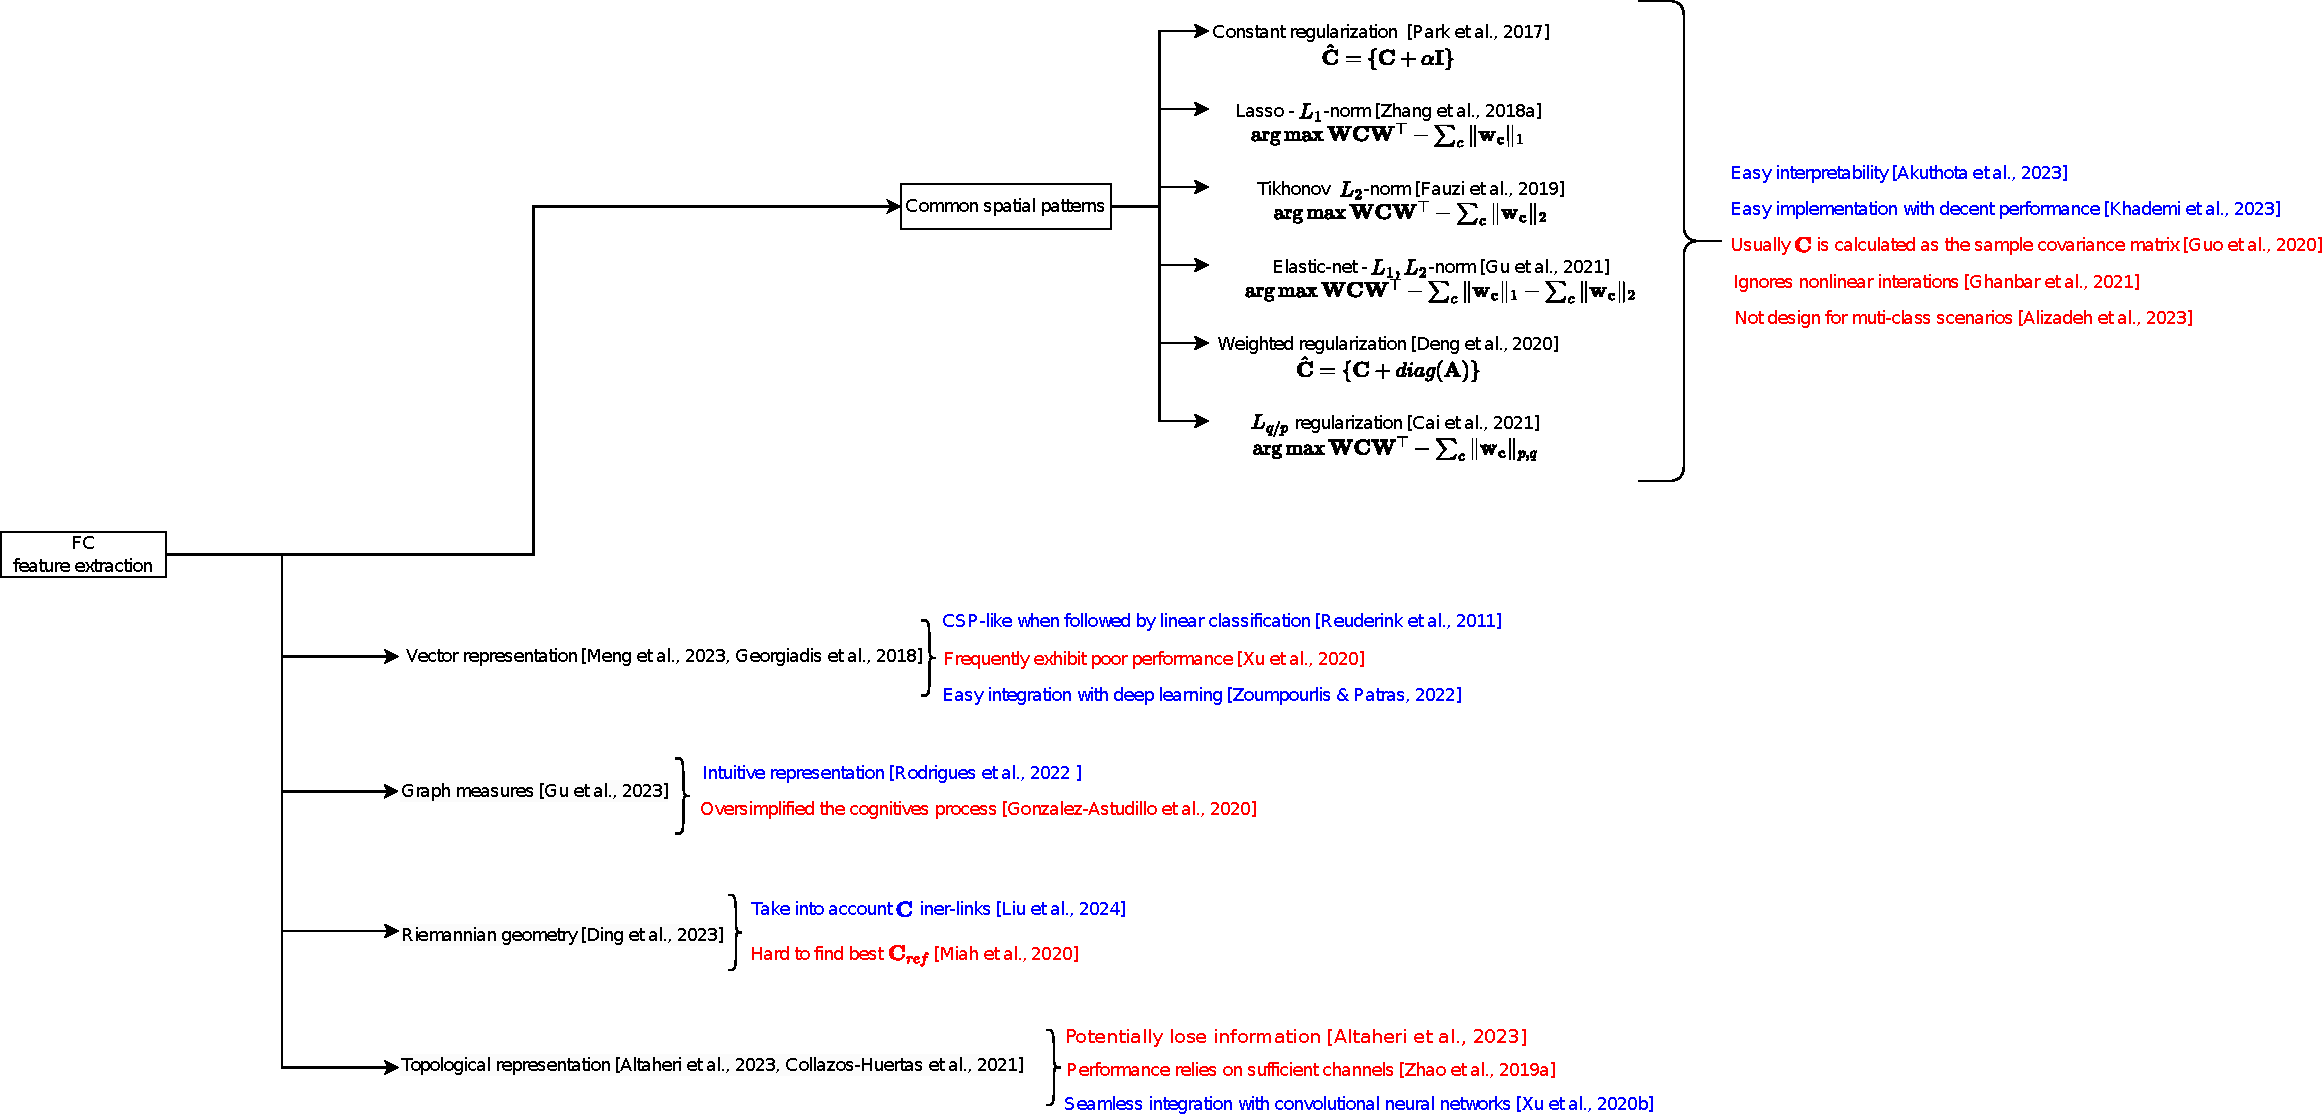
\includegraphics{Figures/state_of_art/sota1_FE}}
        \caption{Four feature extraction approaches for decoding FC in EEG-based MI-BCI: common spatial patterns, FC vectorization, topological representations, and Riemannian geometry \label{fig:sota1_FE}}

\end{figure}

Undoubtedly, CSP is the most extensive feature extraction technique that typically utilizes the simple correlation adjacency matrix to decode connectivities into distinct features, distinguishing between MI classes \cite{miljevic2022electroencephalographic, guo2020eeg}. While it allows direct interpretability using linear spatial filters, its effectiveness is limited as it relies on sample covariance \cite{akuthota2023eeg, darvish2021correlation}. CSP requires sufficient sample data and is susceptible to noise, leading to spurious connectivities and overfitting \cite{khademi2023review}. Consequently, two main approaches to regularization techniques have been explored. The first involves regularizing the covariance matrix through either constant regularization \cite{park2017filter} or weighted regularization, which impacts each channel differently \cite{deng2020local}. The second approach regularizes the projection matrix $\Vec{W}$, specifically, lasso using the $L_1$-norm \cite{zhang2018new}, Tikhonov with the $L_2$-norm \cite{fauzi2019energy}, Elastic-net combining $L_1$ and $L_2$ norms \cite{gu2021common}, and the $L_{q/p}$ regularization, which applies the $q/p$ norm \cite{cai2021single}. Despite the numerous attempts to mitigate spurious connectivities and overfitting, CSP-based techniques often overlook the nonlinearity interactions between EEG signals \cite{ghanbar2021correlation}. Furthermore, they do not offer a direct multi-class scenario \cite{alizadeh2023multi}. 

Other methodologies, such as vectorizing the adjacency matrix, leverage the symmetry of indirect FC to extract the upper triangular values, which contain insights about the mental state \cite{meng2023rhythmic, georgiadis2018exploiting}. As exhibited in \cite{reuderink2011subject}, it has been demonstrated that when vectorizing is paired with linear classification, it mimics the CSP approach. This strategy allows us to classify directly from the values of the FC matrix. Moreover, vectorizing is easily adaptable to new deep learning approaches, ensuring a seamless integration \cite{zoumpourlis2022covmix}. However, this approach is prone to overfitting and often exhibits poor performance \cite{xu2020tangent}. Since FC can be represented as graphs, various studies have employed graph measures as a feature to differentiate between MI classes \cite{gu2023decoding}. In particular, global measures, such as Characteristic path, global efficiency, and clustering coefficient, alongside node measures like local efficiency, nodal centrality, and degree centrality, have been used as features \cite{desbois2021functional, rodrigues2022can}. Nonetheless, graph measures offer oversimplified brain functioning features, often resulting in weak performance, especially in subjects with noisy EEG signals \cite{gonzalez2020network}.

So far, we have primarily discussed FC representations in Euclidean spaces, which do not account for the internal link interactions between signals in the adjacency matrix. Therefore, Riemannian geometry, which leverages the links between the coefficients of symmetric and positive definite (SPD) matrices, has been proposed \cite{freer2019adaptive}. This particular branch of differential geometry allows each matrix to be represented by a point in the manifold $\cal{M}$, where scalar products can be defined in an Euclidean tangent space \cite{mishra2018novel}. Therefore, the distance between two FC matrices can be approximately measured in this tangent space and be used as a feature to distinguish between two MI tasks \cite{ding2023study}. However, the main drawback of Riemannian geometry is the necessity for a reference matrix, typically obtained from the average of all the adjacency matrices, where minor changes can significantly affect the distance \cite{miah2020motor}.

On the other hand, imaging techniques have gained popularity due to the recent success of convolutional neural networks (CNNs) \cite{xu2020learning}. That is why some studies have used a topological representation of the FC connectivity to benefit from the easy integration with CNNs \cite{collazos2021deep}. While often achieving competitive performance, this approach heavily depends on the number of channels and suffers from potential information loss when projecting the adjacency matrix into a 2D topoplot \cite{zhao2019multi,altaheri2023deep}.

In summary, techniques such as CSP and vectorizing give different methodologies for feature extraction, each with advantages and disadvantages. CSP is a widely recognized extraction strategy that uses a correlation adjacency matrix to find linear spatial filters. However, it heavily relies on sample covariance and is susceptible to noise. Conversely, vectorizing the adjacency matrix lets us classify directly from the FC matrix values and is easily integrated with deep learning approaches. Nevertheless, both methods are susceptible to overfitting, resulting in inferior performance. Riemannian geometry provides a possible solution by allowing each matrix to represent a point on the manifold $\cal{M}$. However, it necessitates a reference matrix, making it sensitive to minor changes. The topological representation of FC connectivity integrates well with convolutional neural networks, often demonstrating competitive performance. However, it heavily relies on the number of channels and can potentially lose information when projecting the adjacency matrix into a 2D topoplot. 


\subsection{Subject-Specific EEG Representation for MI-BCI \label{sec:sota2}}

In recent years, there has been an increase in the number of methodologies introduced to handle the problem of artifacts in EEG-based MI-BCI systems \cite{kotte2020methods}. Techniques such as Canonical Correlation Analysis (CCA), Principal Component Analysis (PCA), and Independent Component Analysis (ICA) have become common tools to remove contaminated components from EEG signals \cite{stergiadis2022bss}. Notably, CCA has been identified as particularly effective in removing various artifacts \cite{rashid2020current,lahane2019review}. In addition, spatial methodologies like Common Average Reference (CAR) and Surface Laplacian (SL) have also been used to reduce noise \cite{uribe2019correntropy}. However, despite the effectiveness of these techniques, they might introduce complications by adding noise into other sensors \cite{mridha2021brain}. This problem occurs because the implemented filter removes the average electrical activity from neighboring sensors, leading to alterations in the original signal information \cite{xu2018wavelet}. \changes{On ther other hand, Deep Learning (DL) strategies have shown no significant difference in testing results between models with and without clasical artifact removing strategies. This suggest that merly using DL models may be sufficient to handle artifcat removal \cite{hassanpour2019novel,altaheri2023deep}}. Generally, DL methods can be subcategorized based on the nature of their inputs, which may be raw EEG data or handcrafted features such as statistical measures, graph measures, spectral images, and topological representations. Furthermore, the input dimension, which could be a vector, matrix, or tensor representation, also contributes to the categorization. The type of architecture employed also serves as a basis for differentiating DL, thus forming groups such as discriminative, representative, and generative models. The following section reviews the strengths and weaknesses of each model class.

\subsubsection{Input Formulation in Deep Learning}

Regarding input formulation, DL techniques can be categorized into models that depend on handcraft-based feature representation or raw EEG signals, as depicted in \cref{fig:sota2_input}. Furthermore, the input can be classified according to its dimensionality, represented as either a vector, matrix, or tensor.

The simplest handcraft method employs either graph measurements or signal statistics, with the input represented as a vector $[N_q]$, where $N_q$ denotes the total number of features \cite{gu2023decoding}. Graph measurements are metrics that capture significant properties of connectivity architectures, such as node degree and cluster coefficient. On the other hand, signal statistics represent fundamental characteristics of the signal, like mean, variance, skewness, and kurtosis. Despite the simple nature of these methods, they tend to oversimplify the complex processes within EEG signals, leading to less accurate performance \cite{gonzalez2020network}.

Spectral image approaches are another classification of techniques in which spectrograms, visual representations of the spectrum of frequencies of a signal as it varies with time, are used to portray the EEG signal as spatial-temporal-frequency images. Numerous methods can be employed to extract the spectrogram as a matrix. These techniques include Empirical Mode Decomposition (EMD), a method that decomposes a signal into intrinsic oscillatory components called intrinsic mode functions \cite{tang2020motor}; PSD, a measure of signal's power content versus frequency \cite{ma2020dwt}; Fast Fourier Transform (FFT), a mathematical technique that transforms a function of time into a function of frequency \cite{hassanpour2019novel}; Wavelet Transform (WT), a mathematical transform used to split up data, functions or signals into different frequency components \cite{ortiz2019new}; Short-Time Fourier Transform (STFT), a technique for determining the sinusoidal frequency and phase content of local sections of a signal as it changes over time \cite{tayeb2019validating}; and Continuous Wavelet Transform (CWT), a tool that allows for the analysis of non-stationary signals at many different scales or sizes \cite{lee2019application}.

Once the spectrogram is derived, several strategies can be executed for its organization, ranging from simple two-dimensional matrices to complex three-dimensional tensors. The possible permutations include but are not limited to the following formats: $[N_c \times N_f]$ \cite{ma2020dwt}, $[N_c \times N_c \times N_t]$ \cite{wang2019stable}, $[N_c \times N_c \times (N_f+N_t)]$  \cite{collazos2023posthoc}, $[N_c \times N_c]$ \cite{kwon2021visual}, $[(N_f + N_c)\times N_t]$ \cite{zhang2020motor}, $[(N_t + N_c)\times N_f]$ \cite{kant2020cwt}, $[(N_t + N_c)\times (N_f + N_c)]$ \cite{alwasiti2020motor}, and $[N_c \times N_f \times N_t]$ \cite{miao2020spatial}. $N_t$ stands for time points, $N_c$ number of channels, and $N_f$ number of filters. The selected arrangement largely depends on the specific requirements of the EEG signal analysis and the complexity of the information to be analyzed. Each organizational structure offers a unique perspective and could be more effective for different tasks or scenarios. Despite this flexibility, it's worth noting that there is a potential loss of information in each representation \cite{altaheri2023deep}

\begin{figure}[h!]
    \centering
    \resizebox{1.0\linewidth}{!}{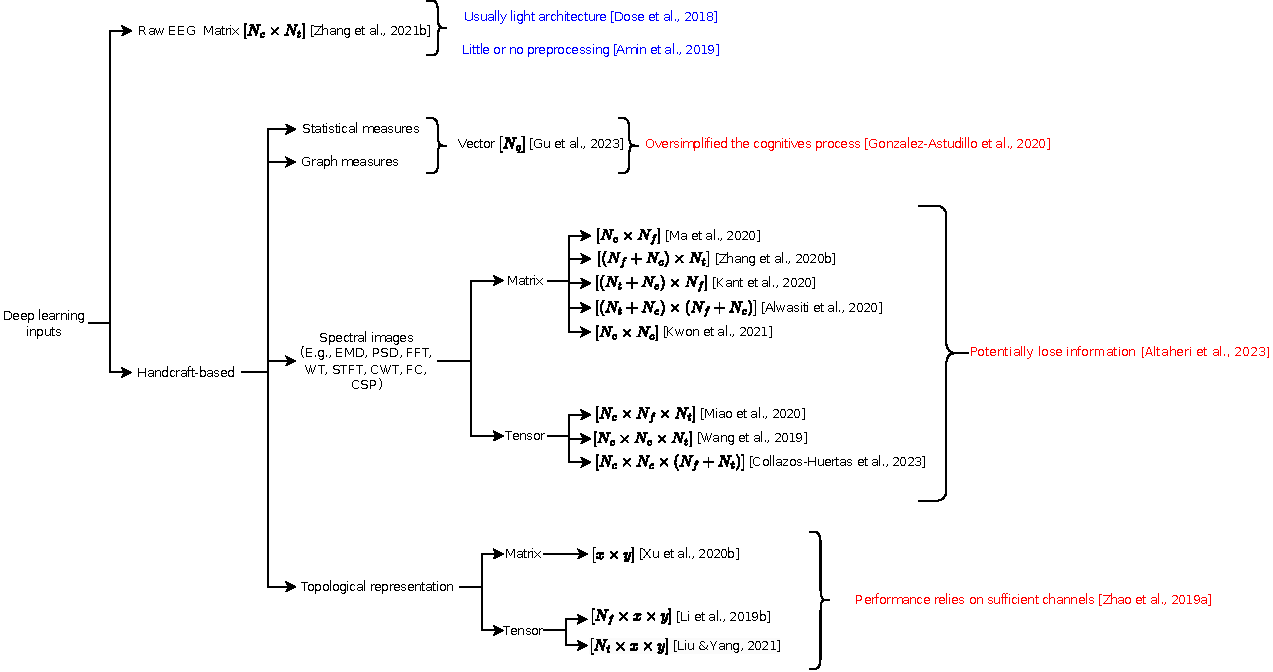
\includegraphics{Figures/state_of_art/sota2_input_v2.pdf}}
        \caption{Deep Learning techniques grouped by input formulation. Featuring handcraft-based feature representation and raw EEG signals, this categorization further divides the input according to dimensions such as vector, matrix, and tensor. The weaknesses and strengths of each form are also highlighted \label{fig:sota2_input}}
\end{figure}

The topological representation approach maps the brain's connectivity to topoplots and then processes them through deep learning architectures. These representations can range from matrix forms to more complex tensor forms. They can appear in the form of a matrix $[x \times y]$ \cite{xu2020learning}, where $x$ and $y$ represent the dimensions of the pixel array in the topoplot image. However, higher dimensional structures are favored to capture the complexities in signal variability across the frequency and time axes. For instance, tensors are often utilized to hold additional dimensions. These structures come in the forms of $[N_f \times x \times y]$ \cite{li2019novel}, and $[N_t \times x \times y]$ \cite{liu2021densely}. These formats offer a more volumetric view of the information in the EEG data. However, it is to be noted that while these approaches can maintain a greater amount of information, they also heavily rely on a sufficient number of channels being available \cite{zhao2019imaging}.

DL models that directly utilize raw EEG data as input are increasingly becoming widespread owing to their unique advantages \cite{dose2018end}. The typical input structure for these models is in the form of a matrix $[N_c \times N_t]$. This configuration allows the model to process the data directly without requiring complex transformations or feature extractions. One of the major strengths of this approach is the lightweight architecture associated with the model. As a result, raw EEG-based DL models are less computationally intensive and require little to no preprocessing \cite{amin2019deep}.

 
\subsubsection{Deep Learning Architectures}

Depending on the underlying architecture, DL models can be categorized into discriminative models, representative models, and generative models, as displayed in \cref{fig:sota2_DLA}. 

Discriminative models encompass architectures such as Multilayer Perceptron (MLP) \cite{amin2019deep}, a type of feedforward artificial neural network model that maps sets of input data onto appropriate outputs. It's worth noting, however, that MLP is relatively inefficient at extracting spatial information \cite{hossain2023status, altaheri2023deep}. Convolutional Neural Networks (CNN) \cite{zhang2021adaptive} represent another type of discriminative model. Like the connectivity pattern between neurons in the human brain, CNNs process data using a grid-like topology. This architecture is particularly apt for automatic spatial, temporal, and spectral filtering \cite{kollHod2023deep}. Furthermore, CNNs readily integrate with other architectures \cite{sharma2023recent}. Discriminative models also include Recurrent Neural Networks (RNN), which utilize previous model states in current inputs. RNNs branch into Long Short-Term Memory (LSTM) units \cite{kumar2019brain} and Gated Recurrent Units (GRU) \cite{luo2018exploring}. LSTM networks, by using gates, can selectively filter temporal information to effectively capture longer dependencies. On the other hand, GRU is a variation of LSTM with only two gates and fewer parameters. Despite these advantages, such networks can lead to inefficiencies when used independently \cite{kostiukevych2021convolutional} and can still face vanishing gradient issues \cite{gao2022parallel}. Graph Neural Networks (GNN), tailored specifically for MI-BCI \cite{ju2023graph}, have emerged recently. These networks extend the concept of Neural Networks (NNs) to graph-structured data, typically involving complex architectures \cite{kulatilleke2023towards}.

\begin{figure}[h!]
    \centering
    \resizebox{1.0\linewidth}{!}{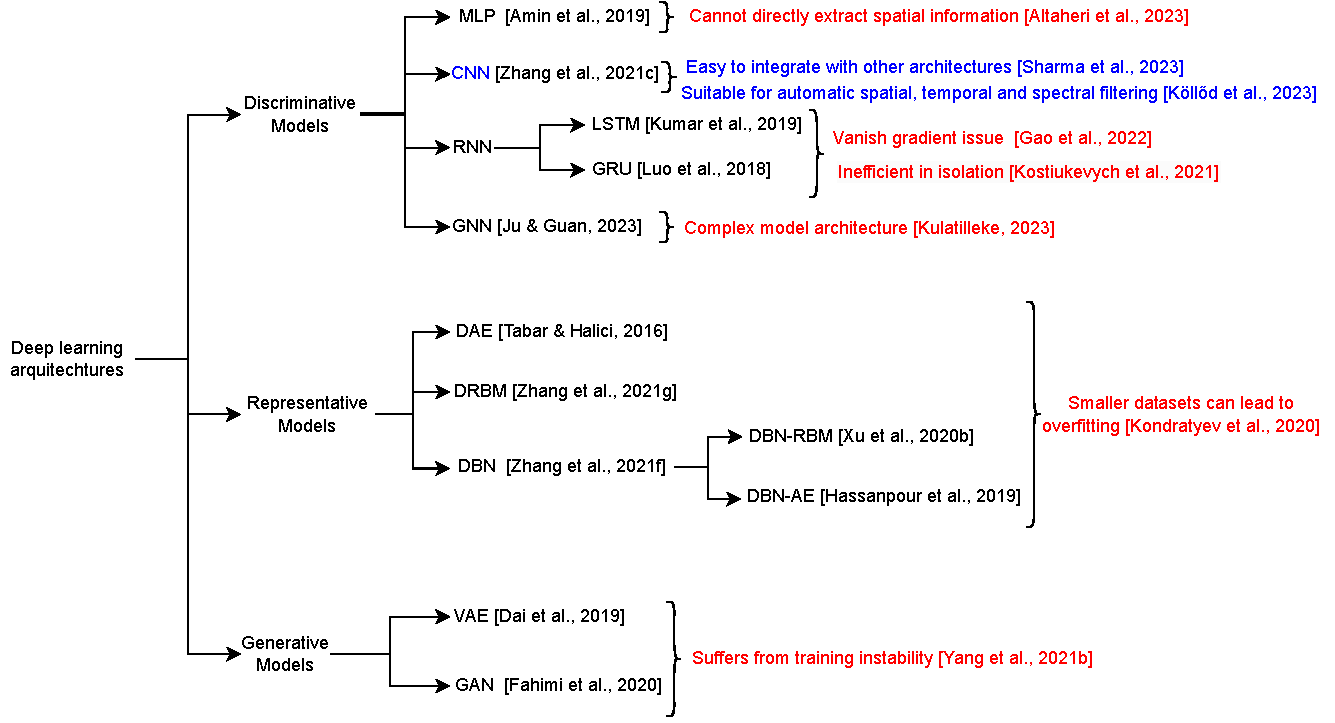
\includegraphics{Figures/state_of_art/sota2_DLAV2.pdf}}
        \caption{Deep learning model categories sorted into discriminative, representative, and generative groups, showcasing their weaknesses and strengths \label{fig:sota2_DLA}}
\end{figure}

Concerning representative models, architectures such as Deep Autoencoders (DAE) \cite{tabar2016novel}, Deep Restrictive Boltzmann Machines (DRBM) \cite{zhang2021survey}, and Deep Belief Networks (DBN) are included~\cite{zhang2021combination}. DAE is a specific variant of a Stacked autoencoder and one of the pioneering deep learning techniques. DBN is a generative probabilistic model with deep architecture that contains many layers of hidden units, and DRBN is a deep learning model capable of learning complex temporal behavior. DBN can further be integrated with autoencoders DBN-AE \cite{hassanpour2019novel} and restrictive Boltzmann machines DBN-RBM \cite{xu2020recognition}. However, These models are prone to overfitting with small datasets \cite{kondratyev2020data}.

Generative models such as Variational Autoencoders (VAE) \cite{dai2019eeg} and Generative Adversarial Networks (GAN) \cite{fahimi2020generative} are also prevalent among DL architectures. VAEs are extensions of traditional autoencoders that learn to encode input data into a set of parameters from which data can be generated, while GANs consist of two networks, a generator and a discriminator, that compete against each other to become more accurate in their predictions. However, GANS and VAE suffer from training instability \cite{yang20214}.

Finally, hybrid architectures integrated from different models have also been developed to exploit the strengths of different models and mitigate their weaknesses, In practice, hybrid methods for EEG-based MI-BCI syetms include CNN+LTSM \cite{zhang2021hybrid}, GAN + CNN \cite{zhang2020data}, LSTM+SVM \cite{kumar2021opticalb}, CNN+SVM \cite{alazrai2019deep}, GNN+CNN \cite{tang2023graph}, and DBN + CNN \cite{dai2019eeg}. to note that CNN is the most relevant architecture being used for most of the hybrid approach since they can extract relevant spatial, temporal, and spectral features.


\subsection{Interpretability Strategies in MI-BCI \label{sec:sota3}}

To enhance the interpretability of models in MI-BCI systems that handle multiple domain features, the primary goal is to unmask the complexity underlying deep learning models and leverage this knowledge to improve model predictions. As shown in \cref{fig:sota3_methods}, XAI methodologies can generally be divided into two categories: post-hoc and intrinsic. 

\begin{figure}[h!]
    \centering
    \resizebox{1.0\linewidth}{!}{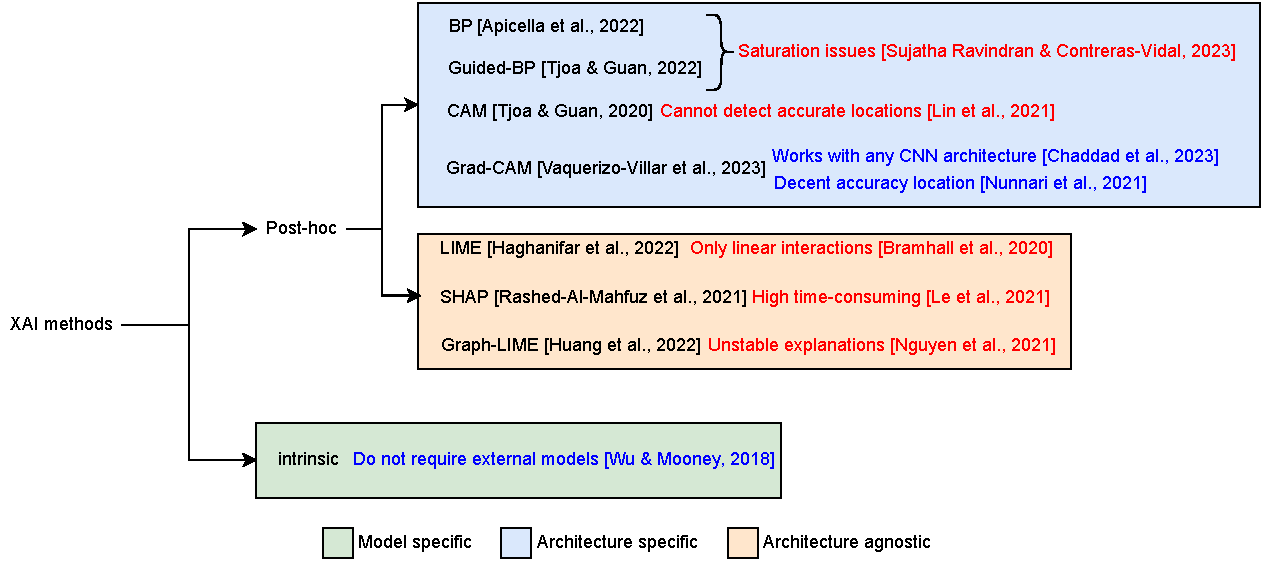
\includegraphics{Figures/state_of_art/sota3_methods.pdf}}
        \caption{Explanability strategies for machine learning and deep learning approaches\label{fig:sota3_methods}}
\end{figure}

Intrinsic models, characterized by their explicit model structures and inherent interpretability, include logistic/linear regression, Random Fourier Features (RFF), k-Nearest Neighbors (KNN), and Bayesian methods \cite{chaddad2023survey}. These techniques directly offer interpretability and do not require external models, but they are model-specific \cite{wu2018faithful}. 

In contrast, post-hoc methods aim to interpret existing models' outputs, serving as a key link between machine predictions and human comprehension \cite{speith2022review}. These methods are further subdivided into architecture-agnostic and architecture-specific approaches. 

Architecture-agnostic interpretation methods work toward creating simple, interpretable approximations of predictive models. They can be applied across many machine learning models without specific prerequisites. These methods focus on understanding a model's behavior and pinpointing the key factors that contribute to their predictions. An example is LIME \cite{haghanifar2022covid}, which offers interpretability but is limited to only linear interactions \cite{bramhall2020qlime}. Another method, SHAP \cite{rashed2021deep}, assigns each feature an importance value for a given prediction, providing a unified measure of feature importance. However, it can be computationally intensive and time-consuming \cite{le2021machine}. Lastly, Graph-LIME \cite{huang2022graphlime} provides explanations based on graph theory but may generate unstable explanations \cite{nguyen2021evaluation}.

Conversely, architecture-specific interpretation methods are custom-shaped to fit particular architectures. The latter leverages shared structural elements among a subset of models \cite{selvaraju2017grad}. For instance, Backpropagation (BP) \cite{apicella2022toward} is commonly utilized as an interpretation method, but it can succumb to saturation issues~\cite{sujatha2023empirical}. Likewise, Guided Backpropagation (Guided-BP) \cite{tjoa2022evaluating} is another architecture-specific method but shares similar challenges with BP methods.

In addition, Class Activation Mapping (CAM) \cite{tjoa2020survey} aims to emphasize influential regions within classification tasks but struggles with precise localization \cite{lin2021you}. The Gradient-weighted Class Activation Mapping (Grad-CAM) method \cite{vaquerizo2023explainable} ameliorates this issue and provides decent location accuracy \cite{chaddad2023survey, nunnari2021overlap}. However, CAM-style methods, including Grad-CAM and its variants, are traditionally limited to a network's final layers \cite{jiang2021layercam, selvaraju2017grad, chattopadhay2018grad}. Gradient-based methods like Grad-CAM often yield noisy maps, limiting interpretability \cite{omeiza2019smooth}. While perturbation-based techniques provide insights, they are computationally intensive \cite{fong2017interpretable}. CAM methods offer single-sample visual explanations but are dependent on model architecture \cite{wang2020score}. Layer CAM, an enhancement of Grad-CAM, offers better input region localization but may overlook important information from earlier layers. \cite{jiang2021layercam}

On the other hand, quantitative explanations are essential for evaluating the performance of XAI models and comparing them numerically \cite{hassija2023interpreting}. Metrics such as Average drop $\%$, increase confidence $\%$, and win $\%$ can be used to measure the quality of explanations and identify the strengths and weaknesses of different XAI methods \cite{naidu2020cam}. This allows researchers to develop more accurate and interpretable XAI models that can be used to solve a wider range of problems.

In conclusion, each interpretability method has its strengths and limitations and provides unique insights into the inner workings of machine learning models \cite{rahate2022multimodal}. Therefore, the choice of an interpretability method should mirror each application's specific requirements and constraints.

\subsection{Summary}

In general, nonlinear methods for extracting indirect functional connectivity data from trial-based EEG signals achieve acceptable accuracy. However, their complexity makes them susceptible to noise, resulting in spurious connectivity. Meanwhile, DL methods capably handle artifacts and EEG representations, necessitating minimal preprocessing. Specifically, models based on CNNs are well-suited for automatic spatial, temporal, and spectral filtering. Furthermore, incorporating intrinsic and post-hoc interpretability strategies into these models could enhance their transparency and interpretability.